\chapter{Rezultati}
\section{Delitev podatkov}
Za končno raziskavo smo izbrali posnetke serij 3, 7 in 11 iz MMID. Vsaka serija vsebuje 109 posnetkov, vsak posnetk 30 primerov stanj, vse skupaj smo jih pridobili 9854. Primere stanj smo skrčili na enakomerno razporeditev, z 2456 primeri vsakega stanja. Sami smo posneli neka minut posnetkov. Vse skupaj 250 primerov stanj, ki smo jih skrčili na enakomerno razporeditev, 62 primerov vsakega stanja. Za učenje nevronskih mrež smo uporabljali množice za učenje z 75\% podatkov in množice za testiranje z 25\% podatkov. Podatki so bili naključno razporejeni med učno in testno množico. Ker smo podatke delili naključno, se lahko posnetki stanj enega prostovoljca pojavijo v učni in testni množici. Pri dodatnem učenju mreže smo uporabili posnetke ene osebe za učenje in testiranje. To skupaj pomeni da sistem ne deluje medosebno. 

\section{Izbira metode povezljivosti}
Ker je kompleksni Pearsonov korelacijski koeficient(CPCC) izračunan iz analitičnih signalov ga lahko definiramo samo za ozke frekvenčne pasove. Pri računanju Grangerjevega indexa vzročnosti(GC) te omejitve ni, tako da smo ga lahko računali na celotnem frekvenčnem območju do 45Hz. Prav tako se je pojavilo vprašanje koliko dolgo epoho EEG signala bomo potrebovali za uspešno razvrščanje. Kot možnosti smo vzeli prvo sekundo, prvi dve sekundi, drugi dve sekundi in prve štiri sekunde po dogodku. Točnost razvrščanja smo ocenili z zgoraj navedeno nevronsko mrežo. Za najboljšo metodo se je izkazal kompleksni Pearsonov korelacijski koeficient na območju 13-30Hz z najdalšimi epohami, 4s. Celotno območje primerjav razvidno iz slike \ref{slika:primerjava_obmocij}.
\begin{figure}
    \begin{center}
    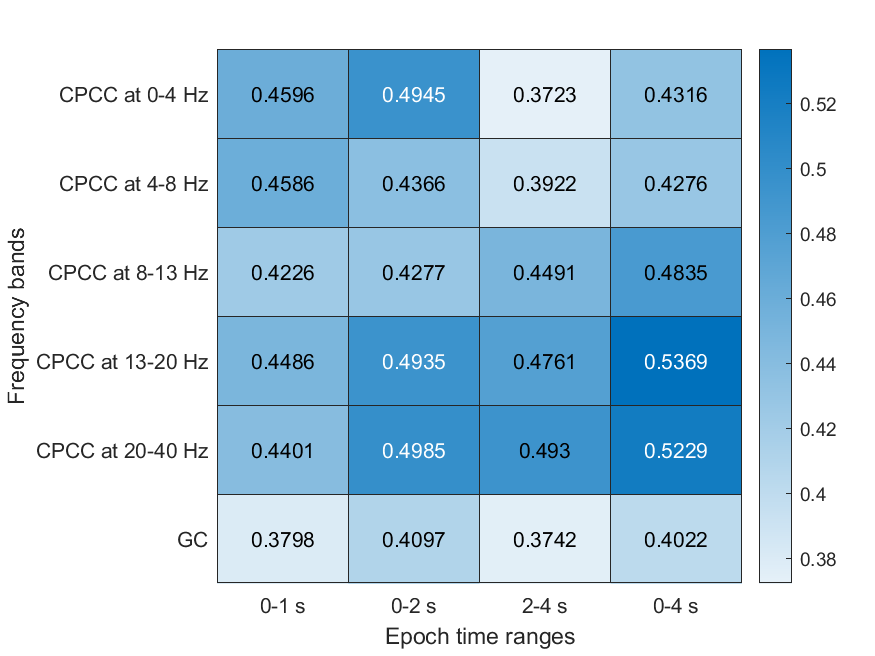
\includegraphics[width=1\linewidth]{slike/Comparison.png}
    \end{center}
    \caption{Točnost razvrščanja po frekvenčnih območjih in dolžini epoh za CPCC in GC. Od zgoraj navzdol CPCC po pasovih delta, theta, alpha, beta in gamma. Spodnja vrstica Grangerjev index vzorčnosti. Epohe od leve proti desni: prva sekunda, prvi dve sekundi, drugi dve sekundi, prve štiri sekunde.}
    \label{slika:primerjava_obmocij}
\end{figure}

\newpage
\subsection{Izbira uporabljenih filtrov}
Knjižnica EEGLAB vsebuje samo filtre z ničelno fazo, ki filtrirajo naprej in nato nazaj po času, kar v našem primeru ni primerno saj podatke prejemamo sekvenčno. Filtrov z ničelno fazo se ne da uporabiti v realnem času. Podatke smo želeli filtrirati s pomočjo Butterworthovega filtra ki vsebuje stanja. Stanja nam omogočajo filtriranje sekvenčnih podatkov saj preprečijo napako na začetku filtra kjer le ta potrebuje predpostaviti začetno staje vseh signalov 0. Ker filtra nista enakovredna saj prvi ne spreminja faz drugi pa jih zamakne, uporabljena metoda CPCC pa deluje na zamikih faz, smo izvedli dodatno testiranje, da smo preverili če pristop deluje enako učinkovito. Razvrščanje matrik pridobljenih z Butterwothovim filtrom(slika \ref{slika:butterwothov_filter_matrika}) v primerjavi z filtrom z ničelno fazo(slika \ref{slika:nicelna_faza_filter_matrika}) je bila primerljivo točno za frekvenčni pas beta(slika \ref{slika:primerjava_filtrov}) iz česar lahko sklepamo, da je filtriranje z Butterwithovim filtrom primerno.
\begin{figure}
    \begin{center}
    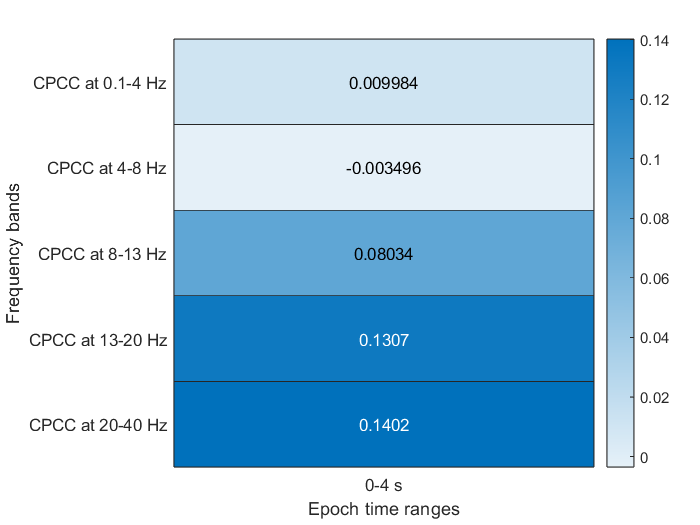
\includegraphics[width=1 \linewidth]{slike/ComparisonFilters.png}
    \end{center}
    \caption{Primerjava točnosti razvrščanja glede na tip filtra. Uporabljena metoda CPCC za epoho prvih štirih sekund za frekvenčne pasove delta, theta, alpha, beta in gamma. Razvrščanje z zgoraj navedeno nevronsko mrežo. Modra predstavlja Butterwothov filter, oranžna predstavlja filter z ničelno fazo.}
    \label{slika:primerjava_filtrov}
\end{figure}

\begin{figure}
    \begin{center}
    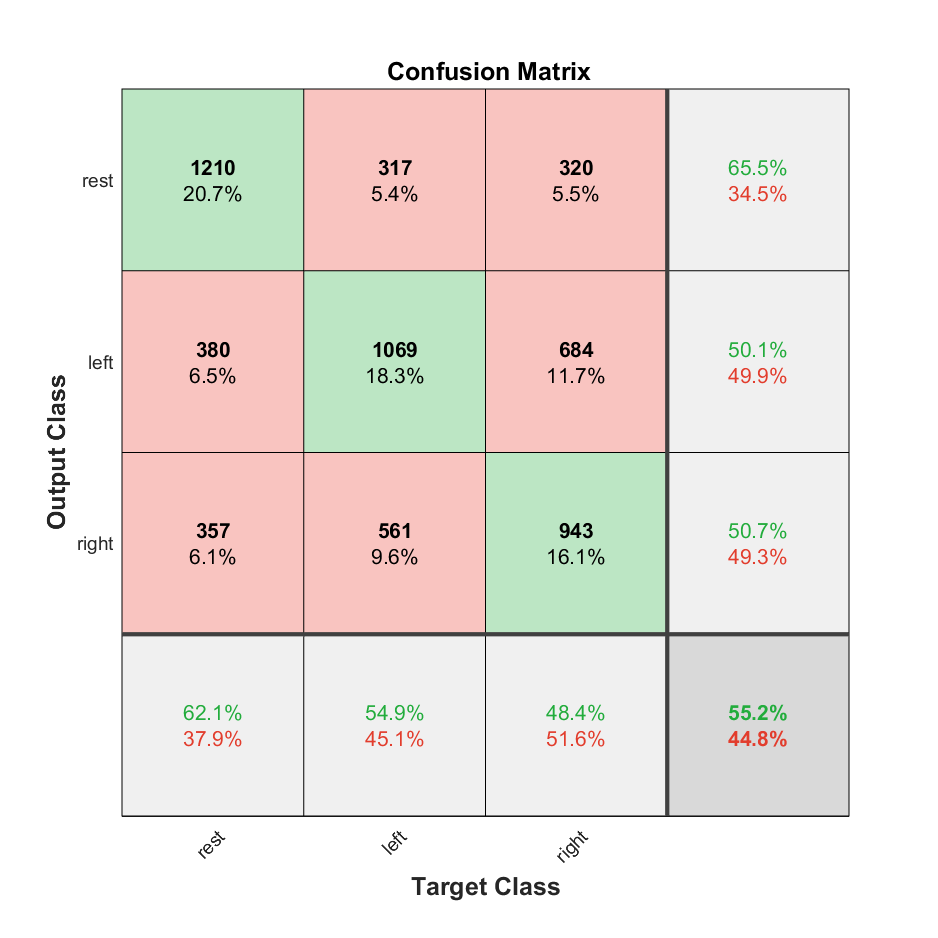
\includegraphics[width=0.8\linewidth]{slike/Confusion eeglabCPCC at 13-20 Hz 0-4 s.png}
    \end{center}
    \caption{Matrika zmede nevronske mreže naučene na podatkih fitriranih s filtrom z ničelno fazo.Uporabljena metoda CPCC za epoho prvih štirih sekund za frekvenčni pas beta. V zelenih poljih vidna točnost za posamezna stanja. Od zgoraj navzdol: skrčena desna pest, skrečena leva pest, stanje mirovanja. }
    \label{slika:nicelna_faza_filter_matrika}
    \end{figure}
    
\begin{figure}
    \begin{center}
    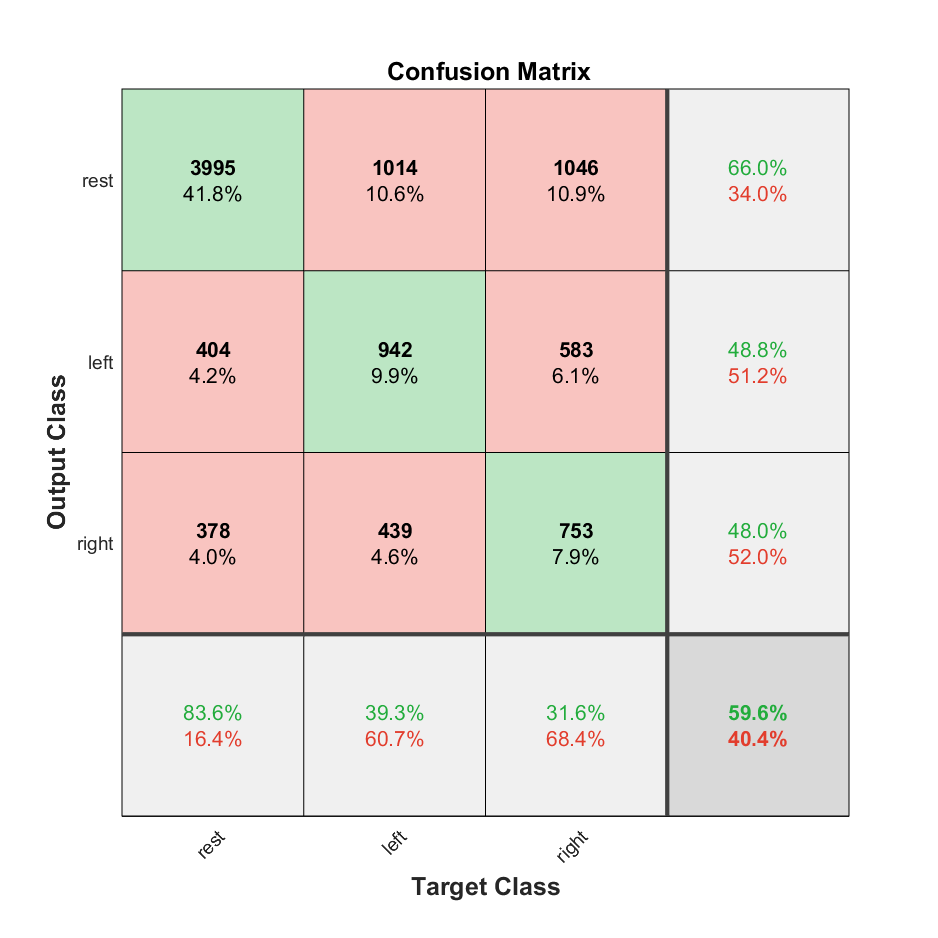
\includegraphics[width=0.8\linewidth]{slike/Confusion my CPCC at 13-20 Hz.png}
    \end{center}
    \caption{Matrika zmede nevronske mreže naučene na podatkih fitriranih z Butterworthovim filtrom. Uporabljena metoda CPCC za epoho prvih štirih sekund za frekvenčni pas beta. V zelenih poljih vidna točnost za posamezna stanja. Od zgoraj navzdol: skrčena desna pest, skrečena leva pest, stanje mirovanja.}
    
    \label{slika:butterwothov_filter_matrika}
    \end{figure}

\section{Rezultati na MMID}
\subsection{Rezulatati z okoljem classification learner}
Z uporabo aplikacije clasifiacation learner smo testirali več načinov razvrščanja. Iz rezultatov predstavljenih v tabeli \ref{tabela:primerjava_tocnosti} lahko razberemo, da so se za najbolj uspešne izkazale metode podpornih vekotrjev(SVM), vendar so te metode računsko zahtevne kar otežuje izvedbo v realnem času. Dober kandidat bi lahko bila odločitvena drevesa saj so enostavna za treniranje in iterpretacijo, vendar so le ta dosegla 41\% točnost. Nevronske mreže ki jih podpira aplikacija so enostavne, vendar pa je njihova interpretacija težja. Dosegle so 49\% točnost.
\begin{table}
\centering
\begin{tabular}{|l|l|c|}
\hline
vrsta razvrščanja & metoda & točnost [\%] \\
\hline SVM&Quadratic SVM&53\\
\hline SVM&Linear SVM&53\\
\hline SVM&Medium Gaussian SVM&53\\
\hline Ensemble&Subspace Discriminant&53\\
\hline SVM&Cubic SVM&52\\
\hline Kernel&SVM Kernel&52\\
\hline Kernel&Logistic Regression Kernel&52\\
\hline SVM&Coarse Gaussian SVM&50\\
\hline Efficient Logistic Regression&Efficient Logistic Regression&49\\
\hline Neural Network&Wide Neural Network&49\\
\hline Neural Network&Medium Neural Network&47\\
\hline Efficient Linear SVM&Efficient Linear SVM&46\\
\hline Neural Network&Trilayered Neural Network&45\\
\hline Neural Network&Bilayered Neural Network&45\\
\hline Naive Bayes&Kernel Naive Bayes&45\\
\hline Neural Network&Narrow Neural Network&45\\
\hline Ensemble&Bagged Trees&44\\
\hline KNN&Coarse KNN&44\\
\hline Ensemble&Boosted Trees&43\\
\hline Ensemble&RUSBoosted Trees&42\\
\hline Tree&Medium Tree&41\\
\hline Tree&Fine Tree&41\\
\hline KNN&Cosine KNN&41\\
\hline Tree&Coarse Tree&41\\
\hline KNN&Medium KNN&40\\
\hline KNN&Weighted KNN&40\\
\hline Ensemble&Subspace KNN&40\\
\hline KNN&Cubic KNN&40\\
\hline KNN&Fine KNN&38\\
\hline SVM&Fine Gaussian SVM&37\\

\hline
\end{tabular}
\caption{Točnost vseh testiranih metod razvrščanja v aplikaciji Clasification Learner.}
\label{tabela:primerjava_tocnosti}
\end{table}

\begin{figure}
    \begin{center}
    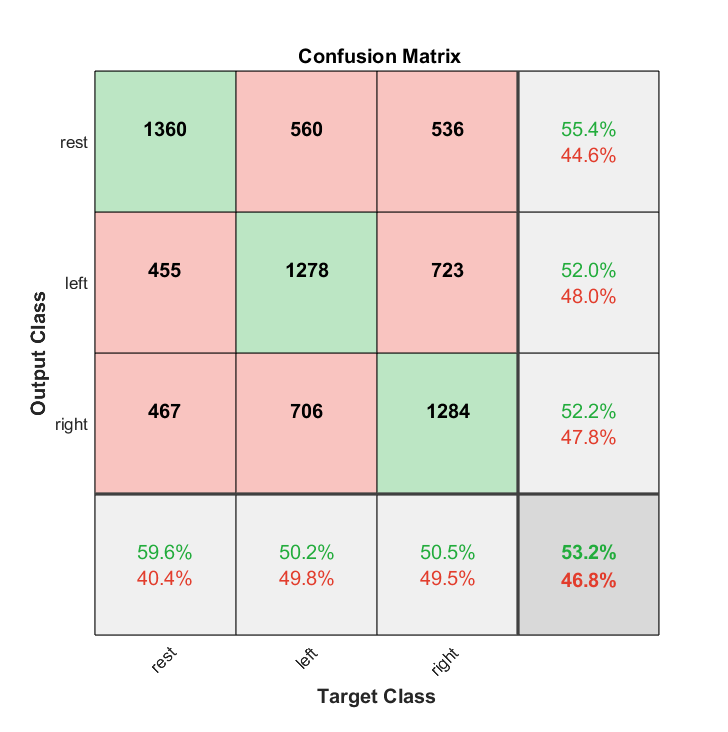
\includegraphics[width=0.8\linewidth]{slike/ConfusionSVM.png}
    \end{center}
    \caption{Matrika zmede metode Quadratic SVM. V poljih vidno število stanj. Od zgoraj navzdol: skrčena desna pest, skrčena leva pest, stanje mirovanja.}
    \label{slika:SVM_matrika}
    \end{figure}

\subsection{Rezultati z uporabo lastne nevronske mreže}
Nato smo poskusili z zgoraj navedeno nevronsko mrežo, ki razvršča matrike povezljivosti. Mreža je dosegla malo višjo točnost kot metode iz aplikacije clasification learner. V primerjavi z najbolšo metodo aplikaije SVM, ki je dosegla 53\% točnost, je mreža dosegla 56\% točnost. Če primerjamo matriko zmede nevronske mreže z matriko zmede metode SVM (sliki \ref{slika:nevronska_mreza_matrika} in \ref{slika:SVM_matrika} ), opazimo, da obe metodi bolj natančno razlikujeta stanje mirovanja od obeh stanj gibanja, medtem ko je razlikovanje med stanji gibanja med seboj manj natančno.

\begin{figure}
\begin{center}
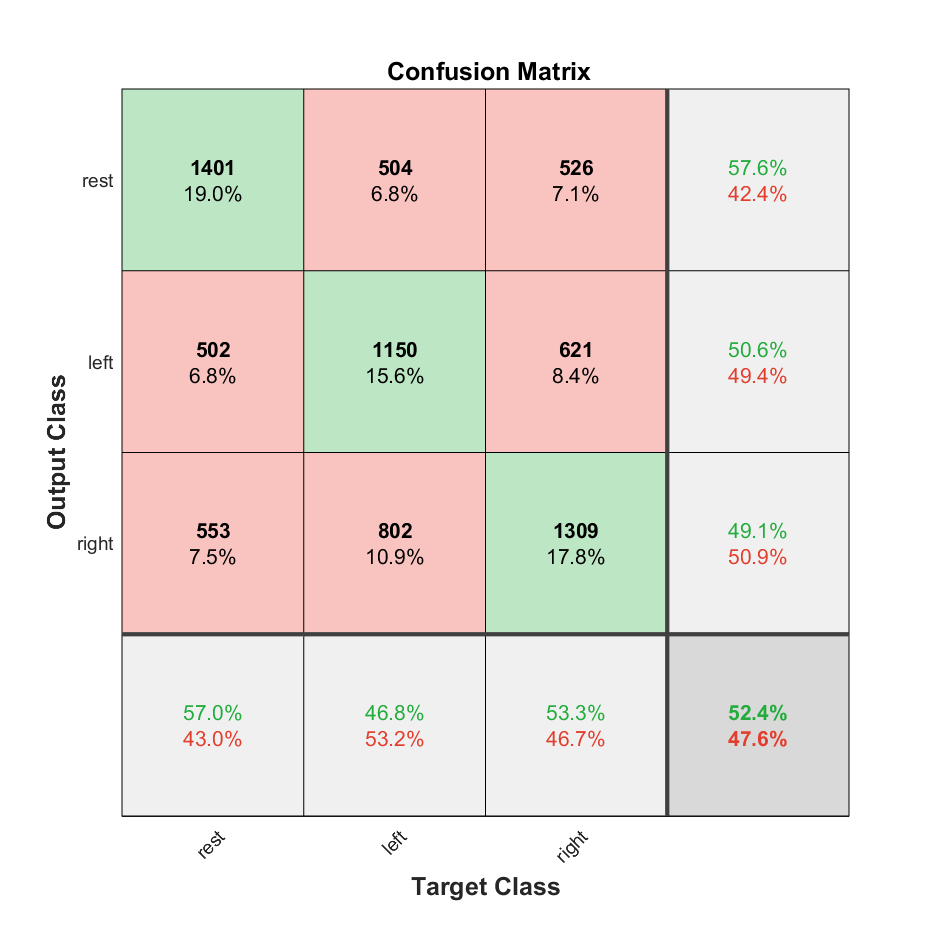
\includegraphics[width=0.8\linewidth]{slike/Confusion_13-20Hz_0s-4s.png}
\end{center}
\caption{Matrika zmede nevronske mreže. V zelenih poljih vidna točnost za posamezna stanja. Od zgoraj navzdol: skrčena desna pest, skrčena leva pest, stanje mirovanja.}
\label{slika:nevronska_mreza_matrika}
\end{figure}



\section{Rezultati na lastnih podatkih}
Da bi se približali pogojem v realnem času, smo nevronsko mrežo dodatno naučili na naših podatkih. Zaradi različnih pogojev snemanja in natančnosti naprav na katerih so podatki snemani je točnost razvrščanja pričakovano padla. Ker nimamo velikega števila posnetkov smo podatke razdelili na pet delov in mrežo natrenirali petkrat. Vsakič smo uporabili en del za testiranje in štiri za učenje. Predstavljeni podatki so seštevek vseh teh testiranj.
\begin{figure}
\begin{center}
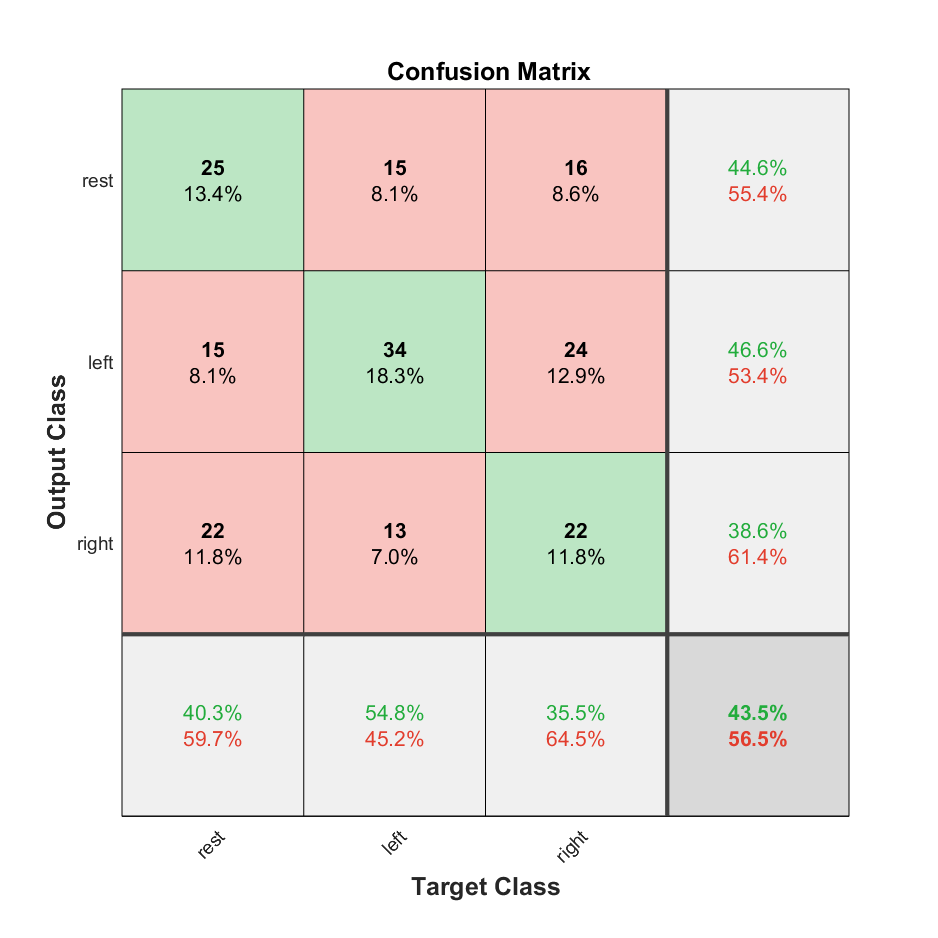
\includegraphics[width=0.8\linewidth]{slike/Confusion_13-20Hz_0s-4s_retrained.png}
\end{center}
\caption{Matrika zmede nevronskih mrež dodatno naučenih na naših podatkih.}
\end{figure}


\section{Preizkus v realnem času}





